\documentclass{llncs}

\usepackage{llncsdoc}
\usepackage{graphicx}
\usepackage{float}
\usepackage{algorithmicx}
\usepackage{algorithm}
\usepackage{algpseudocode}
\usepackage{amsmath,amssymb,stmaryrd}
\usepackage{soul}
\usepackage{color}
\usepackage{tikz}
%\usepackage{subfigure}
\usepackage{subfig}
\usepackage{hyperref}

\newcommand{\LD}{\langle}
\newcommand{\RD}{\rangle}
\def\Rset{\mathbb{R}}
\def\Rsetgeq{\mathbb{R}_{\geq 0}}
\def\Rsetge{\mathbb{R}_{> 0}}

\newcommand{\comment}[1]{{\color{red}{[\sf #1]}}}
\newcommand{\aistis}[1]{{\color{red}{[A: \sf #1]}}}
\newcommand{\taolue}[1]{{\color{red}{[TL: \sf #1]}}}
\newcommand{\dave}[1]{{\color{red}{[D: \sf #1]}}}

\begin{document}

\title{Verifying Team Formation Protocols in PRISM\thanks{This work is supported by
the ERC Advanced Grant VERIWARE.}}
\author{}
\institute{
  Computing Laboratory, University of Oxford\\
  Wolfson Building, Parks Road, Oxford, OX1 3QD, UK
}
\email{}

\maketitle

\begin{abstract}
Multi-agent systems are becoming an increasingly important software paradigm. One of the key advantages of multi-agent systems is that agents can cooperate to achieve certain goals, that requires efficient collaboration protocols of which team formation is a typical example. In this paper we illustrate how probabilistic model checking techniques can be applied for analysis, design and verification of such protocols using the PRISM model checker. To start with, we take a team formation protocol and analyse its performance by modelling as a Discrete-Time Markov Chain. The performance includes the agent organization one and each agent's local one. Then by modelling as a Markov Decision Process we show %what is
the best performance %that can be achieved by the team joining algorithm run by each agent in the protocol.
of running the team joining algorithm individually by each agent in the protocol. Finally we extend such analysis to the competitive coalitional setting using Stochastic Two-Player Games where agents are divided into cooperative and Byzantine ones.
\end{abstract}

\section{Introduction}

\comment{will need a high-level description of PMC in intro, so put this here. Add some comments about complexity}
%

Multi-agent systems have become an important software paradigm. One of the key advantages of multi-agent systems is that agents can cooperate to achieve certain goals, that requires efficient collaboration protocols of which \emph{team formation} is a typical example. In this paper we focus on a typical distributed team formation protocol which was introduced in \cite{gaston2005agent}, where authors used it to analyse the team performance in dynamic networks. The protocol %was studied further in \cite{glinton2008agent}, and
has also been used for analysis of coalition formation for data fusion in sensor networks \cite{glinton2008agent}. The basic setting for the protocol consists of an \emph{agent organization}, i.e., a network of interconnected agents which have certain resources. These agents are supposed to form teams to accomplish tasks which are generated periodically and globally advertised to the agent organization. Agents attempt to form teams to accomplish these tasks. The network topology restricts the set of possible agent teams -- for an agent to be on a team, the agent must have a connection with at least one other agent in that team. Tasks are generic in that they only require that a team of agents with the necessary resources is formed to accomplish the specific task. As in \cite{gaston2005agent}, we do not consider the solution process, but only the team formation.


%In general, \emph{probabilistic model checking} is an automated technique for
%the formal verification of systems that exhibit stochastic behavior. It can, for example,
%calculate the likelihood of the occurrence of certain events
%during the execution of a system, and can be useful to establish performance
%measures. It is based on the construction and analysis of a
%mathematical model of the system, usually from a specification
%in some high-level description language. This model
%generally comprises a set of states, representing all the possible
%configurations of the system, the transitions that can
%occur between these states, and information about when and
%with what probability each transition will occur, and a probabilistic model checker applies algorithmic techniques to analyze the state space and calculate performance measures.
Probabilistic model checking is a formal verification technique
for the analysis of stochastic systems. It is based
on the construction of a probabilistic model from a precise,
high-level description of a system's behaviour. A quantitative
analysis of this model is then performed, by applying a
combination of exhaustive search techniques and numerical
solution methods. In this paper we investigate how probabilistic model checking techniques can be applied for analysis, design and verification of team formation protocols. The majority of existing analyses of such protocols are based on discrete-event simulation. In contrast, probabilistic model checking provides both an exhaustive search of all possible behaviours of the system, including best- and worst-case scenarios, and exact, rather than approximate, quantitative results. Of course, a trade-off inevitably exists. Simulation-based approaches are scalable to much larger and more complex models, at the expense of exhaustiveness and numerical accuracy. The intention of this work is not to show that model checking is ``better" than simulation-based approaches, but rather to highlight that model checking can be used in conjunction with simulation to provide additional insights into a system. As inherently behaviour of distributed protocols is notoriously difficult to understand precisely, formally analysing a small system can be of great help to obtain a better insight into the behaviour of the large system.

\comment{TL: the above paragraph is toooooooooooooooooooooooooooooooooooo long?}

\paragraph{Contributions.} We apply probabilistic model checking techniques to analyse a team
formation protocol \cite{gaston2005agent} using the PRISM model checker \cite{KNP11} with respect to
a given agent organization. Firstly, we model the original version of the protocol using Discrete Time Markov Chain (DTMC), where the behaviour of each agent is described entirely in a probabilistic (deterministic) way. Then we allow agents to make decisions nondeterministically instead of purely probabilistically when forming teams, such systems are naturally modeled by Markov Decision Processes (MDPs). By analysing the MDP we can obtain the best- and worst-case performance of agent organisations. However, MDP only allows fully collaborative behaviours, whereas in many scenarios it is desired for analysis to allow for hostile behaviour of some agents in the organisation. To cater for this we use Stochastic Two-Player Game (STPG) as a model for the system containing two groups of agents -- collaborative and Byzantine, which try to respectively maximise or minimise the performance of the organisation. In all of these three models the performance of an agent organisation or individual agents is analysed by model checking PCTL formulae.

Our experiments illustrate several aspects of agent organisation analysis. As a typical case, we choose four network topologies each consisting of five agents, i.e., fully connected, ring, start, and a network having one isolated node. For each one, we compute the expected performance of the organisation and find organisation-optimal resource allocation among agents. Then we show using MDP model checking what is the best performance that can be achieved by this organisation in two settings, \emph{offline} and \emph{online}, depending on whether the tasks are generated respectively \emph{before} and \emph{after} teams have formed. Then we take the model to STPG setting to obtain the optimal coalitions of different sizes and evaluate their performance.

\comment{resource v.s. skill?}

\comment{add several advantages of our approach - base on results. }




\paragraph{Related work.}


Cooperative behaviour being one of the greatest advantages of the agent based computing has been studied from many different angles over the years. Coalitional games traditionally have been analysed from game-theoretic perspective \cite{osborne1994course}, but in recent years has attracted a lot of attention from researchers in artificial intelligence, especially in cooperative task completion \cite{shehory1998methods}. Several approaches for team formation and collaborative task solving are considered including team formation under uncertainty using simple heuristic rules \cite{kraus2003coalition}, reinforcement learning techniques \cite{abdallah2004organization}, and methods using distributed graph algorithms \cite{manisterski2006forming}. To reason formally about cooperative games several several logics  including Coalitional Game Logic \cite{agotnes2009reasoning} and Strategy Logic \cite{chatterjee2007strategy}, and other formalisms one example of which is Cooperative Boolean Games \cite{dunne2008cooperative} have been introduced and used to analyse coalitional behaviours \cite{bonzon2007efficient}. Model checking has been used to analyse a variety of mutli-agent protocol, i.e. clock synchronisation in wireless sensor networks using Uppaal \cite{heidarian2009analysis}, Gossip  \cite{KNP08d} and Byzantine agreement protocols  \cite{KN02} using PRISM   \cite{KNP11}. MCMAS model checker has been applied to verification of knowledge-based properties in multi-agent systems and classic problems like dining cryptographers \cite{lomuscio2006mcmas}.



\paragraph{Structure.}


\section{Preliminaries}

%In this paper, we shall us discrete-time
%Markov chains (DTMCs), Markov decision processes (MDPs), and Stochastic Two-Player Games (STPGs) as the modeling %formalism. %where time is modelled as
%%discrete steps and the probability of making each transition
%%is given by a discrete probability distribution.
%Below we give a short introduction on these models.

%----------------------------------------------------------------------------------------------------------------

\subsection{Probabilistic Models}

We begin with a brief introduction to the three different types of probabilistic models
that we will use in this paper.

%\vskip5pt
\emph{Discrete-time Markov chains} (DTMCs) are the simplest of these models.
A DTMC $(S,\mathbf{P})$ is defined by a set of states $S$ and a probability transition matrix
$\mathbf{P} : S\times S \rightarrow [0, 1]$, where $\sum_{s'\in S} \mathbf{P}(s, s') = 1$ for all $s \in  S$.
This gives the probability $\mathbf{P}(s, s')$ that a transition will take place from state $s$ to state $s'$.

%\vskip5pt
\emph{Markov decision processes} (MDPs) extend DTMCs by incorporating \emph{nondeterministic choice}
in addition to probabilistic behaviour.
An MDP $(S,Act,Steps)$ comprises a set of actions $Act$
and a (partial) probabilistic transition function $Steps:S\times Act\rightarrow Dist(S)$,
which maps state-action pairs to probability distributions over the state space $S$.
In each state $s\in S$, one or more distinct actions can be taken and, assuming that action $a\in Act$ is chosen,
the distribution $Steps(s,a)$ gives the probability of making a transition to each state.

%Markov Decision Processes (MDP) allow accurate modelling of systems which exhibit
%both probabilistic and nondeterministic behavior. Formally, a Markov decision process (MDP) is a tuple $(S, s_0, Act, %Steps)$ where $S$ is a finite set of states,
%$s_0$ is the initial state, $Act$ is a set of actions
%and $Steps\subseteq S \times Act \times Dist(S)$ is a probabilistic transition relation.
%An MDP transition $s\stackrel{a,\mu}s'$ is made from a state $s\in S$ first by nondeterministically
%selecting an action-distribution pair $(a, \mu)$ such that $(s, a, \mu) \in
%steps$, and second by making a probabilistic choice of the target state $s'$ according to the distribution
%$\mu$, such that $\mu(s') > 0$. A path represents a particular

%An \emph{adversary} represents a particular resolution
%of nondeterminism only. Formally, an adversary of a MDP is a function $A$
%mapping every finite path $\pi$ to a pair $(a, \mu)$ such that $(last(\pi), a, \mu)\in Steps$.
%The evolution of the MDP according to a particular adversary $A$ is a
%measurable set of infinite paths associated with $A$, which can classically be
%provided with a probability measure.

%\vskip5pt
\emph{Stochastic two-player games} (STPGs) generalise MDPs by allowing the nondeterministic choices
in the model to be resolved by two distinct players.
An STPG is a tuple $(S,(S_1,S_2),Act,Steps)$
where the set of states $S$ is partitioned into two disjoint subsets $S_1$ and $S_2$.
As for MDPs, $Steps:S\times Act\rightarrow Dist(S)$ is a function mapping
state-action pairs to distributions over states.
This is a \emph{turn-based} game. In each state $s$ of the game,
either player 1 or player 2 selects an action $a\in Act$,
depending on whether $s$ is in set $S_1$ or $S_2$.

For all three classes of models, we also consider \emph{rewards},
which can be used to capture a variety of additional quantitative measures
(e.g. ...)
For consistency, we assume a simple state-based scheme
i.e. a \emph{reward function} $\rho:S\rightarrow\Rsetgeq$.
\dave{might move rewards to next sect}

%----------------------------------------------------------------------------------------------------------------

\subsection{Probabilistic Model Checking \& PRISM}

Probabilistic model checking involves the construction and analysis of a probabilistic model.
Typically, a high-level description language is used to model a system
(here, we will use the PRISM \cite{KNP11} modelling language).
Then, one or more quantitative properties are formally specified and analysed on the model.
Usually, probabilistic extensions of temporal logic are used to formalise properties.
In this paper, we use the logic PCTL \cite{HJ94},
extended to include reward-based properties \cite{KNP07a},
which can be used to express properties of both DTMCs and MDPs.
We will also generalise the logic to capture properties of stochastic games.

PCTL extends the well known temporal logic CTL, with a probabilistic ($\tt P$) operator.
Informally, this places bounds on the probability of the occurrence of certain events in the model.
We will illustrate the use of PCTL using some simple examples,
referring the reader to \cite{HJ94,KNP07a} for precise details of the syntax and semantics.
For a DTMC, typical PCTL properties would be:
\begin{itemize}
\item ${\tt P}_{<0.01}[\,\Diamond\,\mathit{fail}\,]$ -
``the probability of a failure occurring is less than 0.01''
\item ${\tt P}_{\geq 0.95}[\,\Diamond^{\leq 60}\,\mathit{end}\,]$ -
``the probability of the protocol completing with 60 time units is at least 0.95''.
\end{itemize}
In fact, in practice, we often use a \emph{quantitative} variant of the ${\tt P}$ operator,
denoted ${\tt P}_{=?}$, which returns the actual probability of an event's occurrence, e.g.:
\begin{itemize}
\item ${\tt P}_{=?}[\,\Diamond\,\mathit{fail}\,]$ -
``what is the probability of a failure occurring?''
\end{itemize}
Whereas in a DTMC it is relatively straightforward to define the probability of the occurrence
of an event (such as $\Diamond\,\mathit{fail}$ or $\Diamond^{\leq 60}\,\mathit{end}$ in the examples above),
for MDPs, we must also take account of the nondeterminism in the model.
The standard approach is to use the notion of
\emph{strategies} (also referred to as \emph{policies}, \emph{schedulers}, etc.).
A strategy resolves nondeterminism in an MDP (i.e. chooses an action in a state),
based on its execution history so far.
For a specific strategy, we \emph{can} define the probability of an event.
Thus probabilistic model checking focuses on a best- or worst-case analysis,
quantifying over all possible strategies.
We will continue to focus on quantitative properties,
which now ask for the \emph{minimum} or \emph{maximum} probability of an event occurring, e.g.:
\begin{itemize}
\item ${\tt P}_{\max=?}[\,\Diamond\,\mathit{fail}\,]$ -
``what is the maximum probability of a failure occurring?''
\end{itemize}
For a stochastic game, the notion of strategy generalises naturally...

Finally, rewards...

\dave{mention alg.s, complexity}

\emph{PRISM} \cite{KNP11} is a probabilistic model checking tool.
It supports several different types of models, including DTMCs and MDPs
(it also supports continuous-time Markov chains and probabilistic timed automata).
For this work, we have built a prototype extension of PRISM that adds support for two-player stochastic games.

...

These models are
described in a high-level language, a variant of reactive modules [2] based on guarded
commands. This is described in more detail in Section....

PRISM accepts specifications in either PCTL, or CSL logic depending on the model
type. The model checker then analyses the model and checks if the property holds in each
state.
The reader is invited to consult the PRISM
web site \cite{} for detailed information and corresponding
publications about all of these.

\iffalse
The basic components of the language are modules and variables. A
system is constructed as a number of modules which can interact with each other.
A module contains a number of variables which express the state of the module,
and its behavior is given by a set of guarded commands of the form:

[] $\langle$guard$>$ \! $\langle$command$>$;

The guard is a predicate over the variables of the system and the command describes
a transition which the module can make if the guard is true (using primed variables
to denote the next values of variables). If a transition is probabilistic, then the
command is specified as:

$\langle prob \rangle$ : $\langle$ command $\rangle$ + ...+ $\langle$ prob$\rangle$ : <command>

\fi


\section{Definitions and Algorithms}

The purpose of this section is to provide definitions of terminology
used throughout this paper and then present the algorithms which will be analysed.

\subsection{Definitions}

We now introduce definitions of \emph{agent organisations}, \emph{tasks}, \emph{teams}, and formulae for computing \emph{rewards} to measure the performance of both individual agents and agent teams.

\begin{definition}[Agent Organisation]
An \emph{agent organisation} is a tuple $O=\langle A, N, R, R_A  \rangle$ where
\noindent
\begin{itemize}
\item $A= \{ a_1,a_2,...,a_n \} $ is a set of agents,
\item $N=\{\{a_i,a_j \}\ :$ ``$a_i$ and $a_j$ are neighbours'' $\}$ is a neighbourhood relation,
\item $R=\{r_1,r_2,\dots,r_k\}$ is a set of resource types, and
\item $R_A=\{R_{a_1}, R_{a_2}, \dots, R_{a_n}\}$ is a set of agent resources where $r_j \in R_{a_i} $ $\iff$ ``agent $a_i$ has a resource $r_j$''.
\end{itemize}
\end{definition}

\begin{definition}[Task]
A \emph{task} $T_i=\{r_i\ :\ $``$r_i$ is required by the task $i$''$\}$ is a set of resources that are required to accomplish $T_i$. By $T=\{T_1, T_2,\dots, T_t\}$ we denote a collection of tasks.
\end{definition}

\begin{definition}[Team]
A \emph{team} of agents is denoted by $M_i=\{a_j\ :\ $``$a_j$ is a member of team $i$''$\}$, and the set of all teams is $M=\{M_1, M_2,\dots , M_m\}$. By $\bar{M} = \bigcup_{1\leq i\leq m} M_i$, we denote the set of all agents that are committed to some team. For $1\leq i\leq m$, $R_{M_i}=\bigcup_{a \in M_i}R_{a}$ is the set of resources the team $M_i$ has. The team $M_i$ is said to be able to accomplish the task $T_j$ iff $T_j \subseteq R_{M_i}$.
\end{definition}

\begin{definition}[Rewards]
For agent $a$, we define two types of \emph{reward}:
\begin{itemize}
    \item Type $W_1$, which rewards the \emph{agent} with 1 point if it is in the team which was able to complete its task after team formation is over; and 0 otherwise. Formally,
    \begin{equation} \label{eq:w1agent}
W_1(a) = \left\{
  \begin{array}{l l}
    1 & \quad \text{if $\exists M_i . a \in M_i \wedge T_i \subseteq R_{M_i}$,}\\
    0 & \quad \text{otherwise,}\\
  \end{array} \right.
\end{equation}

    \item Type $W_2$, which rewards 1 point to the \emph{team} which was able to complete its task, and 0 otherwise. The reward is shared equally between team members.
\begin{equation}
W_2(a) = \left\{
  \begin{array}{l l}
    \frac{1}{|M_i|} & \quad \text{if $\exists M_i . a \in M_i \wedge T_i \subseteq R_{M_i}$,}\\
    0 & \quad \text{otherwise.}\\
  \end{array} \right.
\label{eq:w2agent}
\end{equation}
\end{itemize}


For a set of agents $A$, the rewards are defined accordingly as the total reward achieved by its members, i.e.,
\begin{equation}
 W_1(A) = \sum_{a \in A} W_1(a),
\label{eq:w1organisation}
\end{equation}
\begin{equation}
 W_2(A) = \sum_{a \in A} W_2(a).
\label{eq:w2organisation}
\end{equation}
\end{definition}

\comment{TL: move to next section?}


\subsection{Algorithms}

\comment{TL: shall we say something about the whole protocol to give the readers a general picture?}

In this section we provide pseudocode descriptions of algorithms which we later analyse. During the team formation process, each agent performs as follows:
when it is not committed to any team (meaning that it is available and not assigned to any task), it considers each task in a random order. If a task currently
has no other agents committed to it, it can choose to initiate a team, and does so with a probability equal to the ratio between neighbours that are not committed to any team and total number of neighbours. Formally, the probability that an agent $a$ initiates a team is
\[
IP_a = \frac{|\{ a' \in A\ :\ \{a, a'\} \in N \wedge a' \notin \bar{M}  \}|}{|\{ a' \in A\ :\ \{a, a'\} \in N \}|}.
\label{eq:init_prob}
\]
For team joining, if an agent is eligible for a team, it always join the team. Note that only uncommitted agents can commit to
a new or partially filled task, and committed agents can not
decommit from a given task.
%
%can be in one of three states: \textsc{uncommitted}, \textsc{committed}, or \textsc{active}. An agent in the \textsc{uncommitted}
%state is available and not assigned to any task. An agent in the \textsc{committed} state has selected a task, but the full team to work in the task has not yet formed. Finally an agent in the  \textsc{active} state is a member of a team that has fulfilled all of the skill requirements for a task and is actively working on that task. Upon task completion, agents in the active state return to the uncommitted state.
%The core of the protocol is the \textsc{JoinTeam} algorithm, which is used for each agent in the \textsc{uncommitted}
%state to decide which teams to initiate or join. (The algorithm combines team initiation and team joining.)

%\begin{definition}[Initiation probability]
%The team \emph{initiation probability} for agent $a$ used in Algorithm \ref{alg:join_team_org} is the ratio between neighbours that are not committed to any team and total number of neighbours:
%\begin{equation}
%IP_a = \frac{|\{ a' \in A\ :\ \{a, a'\} \in N \wedge a' \notin \bar{M}  \}|}{|\{ a' \in A\ :\ \{a, a'\} \in N \}|}.
%\label{eq:init_prob}
%\end{equation}
%\end{definition}


In Algorithm \ref{alg:join_team_org} we reproduce the pseudocode of the \textsc{JoinTeam} algorithm introduced in \cite{gaston2005agent}. (It combines team initiation and team joining.) %\textsc{JoinTeam} algorithm is executed separately on each agent whenever it is called.
This algorithm will be modelled and analysed as a DTMC, as we shall see in Section \ref{}.

\begin{algorithm}[H]
\caption{Team joining algorithm \cite{gaston2005agent} (probabilistic and deterministic)}
\label{alg:join_team_org}
\begin{scriptsize}
\begin{algorithmic}
\Procedure{JoinTeam}{$a$, $T$, $M$}
  \ForAll {$T_i \in T$ in random order}
    \If {$a \notin \bar{M}$} \Comment{agent is not committed}
      \If {$|M_i|=0$} \Comment{team for task i is empty}
	\If {$R_a \cap T_i \neq \emptyset$} \Comment{agent has skill (is true if called from \textsc{Online})}
	  \State with probability $IP_a$: $M_i \leftarrow M_i \cup \{a\}$ \Comment{initiate a team (see equation \ref{eq:init_prob})}
	\EndIf
      \ElsIf {$\exists \{a,a'\} \in N . a' \in M_i$} \Comment{there is neighbour in team for task i}
	\If {$R_a \cap T_i \setminus R_{M_i} \neq \emptyset$} \Comment{agent has a missing resource}
	  \State $M_i \leftarrow M_i \cup \{a\}$ \Comment{join team}
	\EndIf
      \EndIf
    \EndIf
  \EndFor
\EndProcedure
\end{algorithmic}
\end{scriptsize}
\end{algorithm}

\comment{TL: the problem of developing or learning effective team initialing and team joining policies is also important ...}

To tackle the problem of finding the best team initialing and team joining strategy, we modify the original \textsc{JoinTeam} algorithm by
allowing agents to make decisions regarding what actions to take, instead of picking one randomly. Technically, the changes are as follows, which
are highlighted in Algorithm \ref{alg:join_team_nondet}.
\begin{itemize}
 \item Remove restriction of considering tasks in random order allowing agent to consider arbitrary task.
 \item Replace probabilistic choice to initiate the team by nondeterministic one.
 \item Allow agent not to join a team even if it has the resource and neighbour in that team.
\end{itemize}

This algorithm allows for the analysis of best-case performance that can be achieved by the protocol and also to analyse the agent organisations with \emph{hostile} agents which try to reduce organisation's performance. It will be modelled and analysed as an MDP and a STPG respectively, as we shall see in Section \ref{}.

\begin{algorithm}[H]
\caption{Team joining algorithm (non-deterministic)}
\label{alg:join_team_nondet}
\begin{scriptsize}
\begin{algorithmic}
\Procedure{JoinTeam}{$a$, $T$, $M$}
  \ForAll {$T_i \in T$ in \hl{arbitrary} order}
    \If {$a \notin \bar{M}$} \Comment{agent is not committed}
      \If {$|M_i|=0$} \Comment{team for task i is empty}
	\If {$R_a \cap T_i \neq \emptyset$} \Comment{agent has skill (is true if called from \textsc{Online})}
	    \State \hl{$M_i \leftarrow M_i \cup \{a\}$  \textbf{or} $M_i \leftarrow M_i$} \Comment{initiate a team or do nothing}
	\EndIf
      \ElsIf {$\exists \{a,a'\} \in N . a' \in M_i$} \Comment{there is neighbour in team for task i}
	\If {$R_a \cap T_i \setminus R_{M_i} \neq \emptyset$} \Comment{agent has a missing resource}
	  \State \hl{$M_i \leftarrow M_i \cup \{a\}$ \textbf{or} $M_i \leftarrow M_i$} \Comment{join a team or do nothing}
	\EndIf
      \EndIf
    \EndIf
  \EndFor
\EndProcedure
\end{algorithmic}
\end{scriptsize}
\end{algorithm}

We observe that there are two natural ways to call \textsc{JoinTeam}: \textsc{Offline} procedure first initiates the set of tasks and then sequentially calls \textsc{JoinTeam} procedures of every agent in random order, which is described in Algorithm \ref{alg:join_team_org}; In contrast, \textsc{Online} routine calls \textsc{JoinTeam} procedures for agents \emph{before} selecting the tasks. We investigate both the offline and the online version of the algorithms because it provides a nice comparison between optimisation against specific tasks (offline version), and distribution of tasks (online version). As we will see in the results section for STPGs, whether offline and online version provides better performance depends on network topology.


\begin{algorithm}[H]
\caption{Offline and online versions of the algorithm}
\label{alg:main_process}
\begin{scriptsize}
\begin{algorithmic}
\Procedure{Offline}{$t$} \Comment{$t$ - number of tasks}
  \State $M = \{M_i = \emptyset\ :\ 1\leq i \leq t\}$ \Comment{initialise empty teams}
  \State $T = \{T_i\neq \emptyset\ :\ T_i \subseteq_{random} R,\ 1\leq i \leq t\}$ \Comment{initialise tasks at random}
  \ForAll {$a \in A$ in random order}
    \State \Call{JoinTeam}{$a$, $T$, $M$}
  \EndFor
  \State perform tasks and compute rewards
\EndProcedure
\Statex
\Procedure{Online}{$t$} \Comment{$t$ - number of tasks}
  \State $M = \{M_i = \emptyset\ :\ 1\leq i \leq t\}$ \Comment{initialise empty teams}
  \ForAll {$a \in A$ in random order}
    \State \Call{JoinTeam}{$a$, $T$, $M$}
  \EndFor
  \State $T = \{T_i\neq \emptyset\ :\ T_i \subseteq_{random} R,\ 1\leq i \leq t\}$ \Comment{initialise tasks at random}
  \State perform tasks and compute rewards
\EndProcedure
\end{algorithmic}
\end{scriptsize}
\end{algorithm}

\section{Models and Experimental Setup}

\subsection{PRISM Models}

\comment{give a small example of PRISM models and explain DTMC, MDP and STPG}

\subsection{Experimental Setup}
\label{subsec:exp_set}
For our experiments we mainly consider organisations consisting of five agents which are organised in four networks: fully connected, ring, start, and a network having one isolated node. Each agent is assigned one resource, and there are three different resources available. For each network we find the optimal resource allocation with respect to task generation described\footnote{We have chosen this way for allocating resources so that we could easily show how the performance can be improved by changing the strategy while keeping actions unchanged (i.e. compare DTMC and MDP models).} below using DTMC model checking (see section \ref{sec:results}). These organisations are then fixed and used in all experiments.

\subsubsection{Agent Organisations.}
We run experiments with a set of five agents $A= \{ a_1,a_2,a_3,a_4,a_5 \} $ and a set of  three resources $R=\{r_1,r_2,r_3\}$ arranged in four different agent organisations (see figure \ref{fig:network_configurations} for graphical representations of the organisations):
\begin{itemize}
 \item Fully connected (figure \ref{subfig:fully_connected}) $O_{fc}=\langle A, N_{fc}, R, R_{A_{fc}}  \rangle$ where
    \begin{itemize}
    \item $N_{fc}=\{\{a_i,a_j \}\ : 1 \le i,j \le 5, i\neq j \}$,
    \item $R_{A_{fc}}=\{R_{a_1}, R_{a_2}, R_{a_3}, R_{a_4}, R_{a_5}\}$ where $R_{a_1}=\{r_1\}$, $R_{a_2}=\{r_1\}$, $R_{a_3}=\{r_2\}$, $R_{a_4}=\{r_2\}$, and $R_{a_5}=\{r_3\}$.
    \end{itemize}
 \item Ring (figure \ref{subfig:ring}) $O_r=\langle A, N_r, R, R_{A_r}  \rangle$ where
    \begin{itemize}
    \item $N_r=\{\{a_i,a_j \}\ : 1 \le i,j \le 5, i\neq j, i\le 5 \implies j=i+1, i=5 \implies j=1 \}$,
    \item $R_{A_r}=\{R_{a_1}, R_{a_2}, R_{a_3}, R_{a_4}, R_{a_5}\}$ where $R_{a_1}=\{r_1\}$, $R_{a_2}=\{r_2\}$, $R_{a_3}=\{r_1\}$, $R_{a_4}=\{r_2\}$, and $R_{a_5}=\{r_3\}$.
    \end{itemize}
 \item Star (figure \ref{subfig:star}) $O_s=\langle A, N_s, R, R_{A_s}  \rangle$ where
    \begin{itemize}
    \item $N_s=\{\{a_i,a_j \}\ : 1 \le i,j \le 5, i\neq j, i=1 \}$,
    \item $R_{A_s}=\{R_{a_1}, R_{a_2}, R_{a_3}, R_{a_4}, R_{a_5}\}$ where $R_{a_1}=\{r_1\}$, $R_{a_2}=\{r_2\}$, $R_{a_3}=\{r_2\}$, $R_{a_4}=\{r_3\}$, and $R_{a_5}=\{r_3\}$.
    \end{itemize}
 \item Isolated agent (figure \ref{subfig:isolated}) $O_{ia}=\langle A, N_{ia}, R, R_{A_{ia}}  \rangle$ where
    \begin{itemize}
    \item $N_{ia}=\{\{a_i,a_j \}\ : 1 \le i,j \le 5, i\neq j, (i=5 \vee j=5) \implies (i=4 \vee j=4) \}$,
    \item $R_{A_{ia}}=\{R_{a_1}, R_{a_2}, R_{a_3}, R_{a_4}, R_{a_5}\}$ where $R_{a_1}=\{r_1\}$, $R_{a_2}=\{r_2\}$, $R_{a_3}=\{r_3\}$, $R_{a_4}=\{r_3\}$, and $R_{a_5}=\{r_2\}$.
    \end{itemize}
\end{itemize}


\subsubsection{Tasks.} \label{subsec:tasks} We fix seven different tasks that will be used in experiments $T=\{\{r_1\},\{r_2\},\{r_3\},\{r_1,r_2\},\{r_1,r_3\},\{r_2,r_3\},\{r_1,r_2,r_3\}\}$. When running the algorithm two tasks $T_1$ and $T_2$ are picked uniformly and independently at random (with replacement) and are advertised to the agent organisation. So there are total of 49 different combinations of $T_1$ and $T_2$ that can be generated.


\begin{figure}[H]
\centering
\subfloat[Fully connected]{
  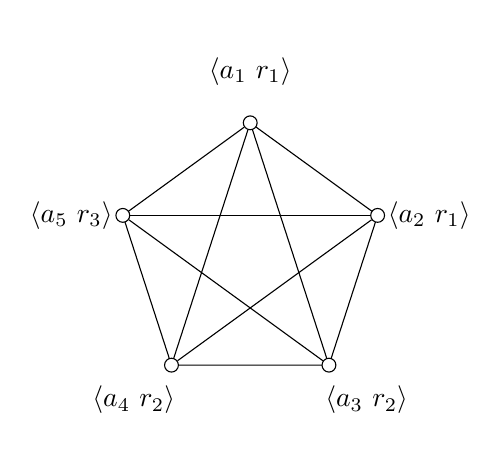
\begin{tikzpicture}
      \tikzstyle{every node}=[draw,circle,fill=white,minimum size=5pt,
			      inner sep=0pt]
      \draw (0,0) 	 node (agent1) [label=90:$\LD a_1\ r_1 \RD$] {}
	  -- ++(-36:2.0cm)   node (agent2) [label=right:$\LD a_2\ r_1 \RD$] {}
	  -- ++(-108:2.0cm) node (agent3) [label=-30:$\LD a_3\ r_2 \RD$] {}
	  -- ++(-180:2.0cm) node (agent4) [label=210:$\LD a_4\ r_2 \RD$] {}
	  -- ++(108:2.0cm) node (agent5) [label=left:$\LD a_5\ r_3 \RD$] {}
	  -- (agent1);
      \draw (agent1) -- (agent3);
      \draw (agent1) -- (agent4);
      \draw (agent2) -- (agent4);
      \draw (agent2) -- (agent5);
      \draw (agent3) -- (agent5);
  \end{tikzpicture}
  \label{subfig:fully_connected}
}\ \ \
\subfloat[Ring]{
  \begin{tikzpicture}
      \tikzstyle{every node}=[draw,circle,fill=white,minimum size=5pt,
			      inner sep=0pt]
      \draw (0,0) 	 node (agent1) [label=90:$\LD a_1\ r_1 \RD$] {}
	  -- ++(-36:2.0cm)   node (agent2) [label=right:$\LD a_2\ r_2 \RD$] {}
	  -- ++(-108:2.0cm) node (agent3) [label=-30:$\LD a_3\ r_1 \RD$] {}
	  -- ++(-180:2.0cm) node (agent4) [label=210:$\LD a_4\ r_2 \RD$] {}
	  -- ++(108:2.0cm) node (agent5) [label=left:$\LD a_5\ r_3 \RD$] {}
	  -- (agent1);
  \end{tikzpicture}
  \label{subfig:ring}
}

\subfloat[Star]{
  \begin{tikzpicture}
      \tikzstyle{every node}=[draw,circle,fill=white,minimum size=5pt,
			      inner sep=0pt]
      \draw (0,0) 	 node (agent1) [label=90:$\LD a_1\ r_1 \RD$] {}
	  -- ++(-36:2.0cm)   node (agent2) [label=right:$\LD a_2\ r_2 \RD$] {}
	   ++(-108:2.0cm) node (agent3) [label=-30:$\LD a_3\ r_2 \RD$] {}
	   ++(-180:2.0cm) node (agent4) [label=210:$\LD a_4\ r_3 \RD$] {}
	   ++(108:2.0cm) node (agent5) [label=left:$\LD a_5\ r_3 \RD$] {}
	  -- (agent1);
      \draw (agent1) -- (agent3);
      \draw (agent1) -- (agent4);
  \end{tikzpicture}
  \label{subfig:star}
}\ \ \
\subfloat[Isolated]{
  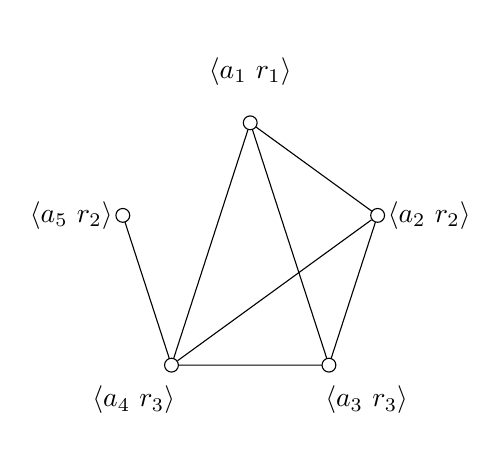
\begin{tikzpicture}
      \tikzstyle{every node}=[draw,circle,fill=white,minimum size=5pt,
			      inner sep=0pt]
      \draw (0,0) 	 node (agent1) [label=90:$\LD a_1\ r_1 \RD$] {}
	  -- ++(-36:2.0cm)   node (agent2) [label=right:$\LD a_2\ r_2 \RD$] {}
	  -- ++(-108:2.0cm) node (agent3) [label=-30:$\LD a_3\ r_3 \RD$] {}
	  -- ++(-180:2.0cm) node (agent4) [label=210:$\LD a_4\ r_3 \RD$] {}
	  -- ++(108:2.0cm) node (agent5) [label=left:$\LD a_5\ r_2 \RD$] {};
      \draw (agent1) -- (agent3);
      \draw (agent1) -- (agent4);
      \draw (agent2) -- (agent4);
  \end{tikzpicture}
  \label{subfig:isolated}
}

\caption{Experimental configurations of the agent organisations with optimal resource allocation (see table \ref{tab:optimal_r}).}
\label{fig:network_configurations}
\end{figure}


\section{Results}
\label{sec:results}

In this section we present results obtained using three models: DTMC, MDP, and STPG. Table \ref{tab:model_sizes} compares model construction information for different sizes of fully connected agent organisations \footnote{We chose fully connected agent organisation because it produces largest models.}: model size in terms of number of states and transitions and construction time. All of the experiments were performed on a 2.8GHz Intel Core 2 PC, 4Gb of RAM running Fedora Core 10 operating system. It is interesting to see that nondeterministic model has a relatively smaller statespace because agent choices do not have to be permuted at model construction stage. However, the model checking is generally more time consuming for MDPs and STPGs than for DTMCs.


\begin{table}
\centering
\subfloat[DTMC]{
\begin{tabular}{ | l | l | l | l |}
    \hline
    Agents & States & Transitions & Const. Time \\ \hline
    2 & 1865 & 2256 & 0.112s  \\ \hline
    3 & 17041 & 20904 & 0.311s \\ \hline
    4 & 184753 & 226736 & 3.347s \\ \hline
    5 & 2366305 & 2893536 & 74.36s \\ \hline
    6 & 35058241 & 42638400 & 2916.235s \\ \hline
\end{tabular}
}
\subfloat[MDP and STPG]{
 \begin{tabular}{ | l | l | l | l |}
    \hline
    Agents & States & Transitions & Const. Time \\ \hline
    2 & 1405 & 1846 & 0.045s  \\ \hline
    3 & 9721 & 12474 & 0.167s \\ \hline
    4 & 76865 & 96664 & 1.109s \\ \hline
    5 & 731233 & 907992 & 5.0536s \\ \hline
    6 & 8155873 & 10040112 & 29.74s \\ \hline
\end{tabular}
}

\caption{Model comparison for different number of agents in a fully connected agent organisation and different models for offline version of the Algorithm \ref{alg:main_process}.}
\label{tab:model_sizes}
\end{table}

As mentioned in Section \ref{subsec:exp_set}, for each topology from Figure \ref{fig:network_configurations} we obtained the optimal resource allocations using PCTL model checking on DTMC model of the offline version of the algorithm (see Algorithms \ref{alg:main_process} and \ref{alg:join_team_org}). The following PCTL formulae were used to compute the expected rewards of the agent organisation under a particular resource allocation:
\[
R_{\{\mbox{``$W_1(O)$''}\}=?} [F \mbox{ ``finished''}]
\]
\[
R_{\{\mbox{``$W_2(O)$''}\}=?} [F \mbox{ ``finished''}]
\]
After obtaining the expected rewards for all possible resource allocations we then selected the ones which have the highest expected reward. The results are summarised in Table \ref{tab:optimal_r}.


\begin{table}[H]
 \centering
 \begin{tabular}{ | l | l | l | l |}
    \hline
    Organisation $O$ & Additional constraints & Example $\LD R_{a_1}R_{a_2}R_{a_3}R_{a_4}R_{a_5}\RD$ \\ \hline
    $O_{fc}$ & - & $R_A=\LD \{r_1\}\{r_1\}\{r_2\}\{r_2\}\{r_3\}\RD$  \\ \hline
    $O_r$ & $R_{a_1}\neq R_{a_5} \wedge \forall i < 5 . R_{a_i} \neq  R_{a_{i+1}} $ & $R_A=\LD \{r_1\}\{r_2\}\{r_1\}\{r_2\}\{r_3\}\RD$  \\ \hline
    $O_s$ & $R_{a_1}=\{r\} \wedge \forall i > 1 . r \notin R_{a_i} $  & $R_A=\LD \{r_1\}\{r_2\}\{r_2\}\{r_3\}\{r_3\}\RD$  \\ \hline
    $O_{ia}$ & $R_{a_5}=\{r\} \wedge \exists i < 4 . r \in R_{a_i} $ & $R_A=\LD \{r_1\}\{r_2\}\{r_3\}\{r_3\}\{r_2\}\RD$  \\ \hline
\end{tabular}
\caption{Optimal resource allocations ($R_A$) for agent organisations from figure \ref{fig:network_configurations} with respect to rewards defined in equations \ref{eq:w1organisation} and \ref{eq:w2organisation}. All allocations satisfy the following constraint $\forall i. |R_{a_i}|=1 \wedge   \forall i.1 \le|\{ R_{a_j} : r_i \in R_{a_j} (1 \le j \le 5 )\}|\le 2$.}
\label{tab:optimal_r}
\end{table}

Please note that the resource allocations from Table \ref{tab:optimal_r}'s example column have been chosen for all future experiments and are shown in Figure \ref{fig:network_configurations}. we have decided to fix resource allocations in this way as it allows us to show how model-checking techniques can be used to improve performance of the algorithm by synthesising strategies (see discussion of MDP results in Section \ref{subsec:MDP}).

\subsection{DTMC}
\label{subsection:DTMC}

\comment{Discuss reward structures, topology differences, gap between min and max agent performance. discuss task completion probabilities, write PCTL formulae. Reference where models can be checker online.}

\begin{figure}
 \subfloat[Reward $W_1(O)$.]{
  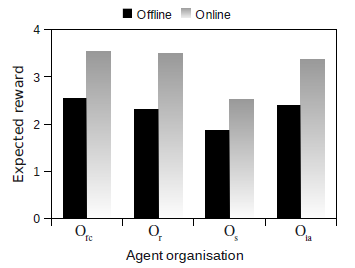
\includegraphics[scale=0.65]{images/W1.png}
}
\subfloat[Reward $W_2(O)$.]{
  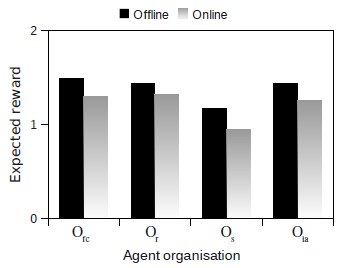
\includegraphics[scale=0.65]{images/W2.png}
}
\caption{Expected rewards for agent organisations when using online and offline (see Algorithm \ref{alg:main_process}) versions of the Algorithm \ref{alg:join_team_org}.}
\end{figure}



\begin{table}
\subfloat[Offline. $W_1$ reward structure.]{
 \begin{tabular}{ | l | l | l | l | l |}
    \hline
    $O$ & $W_1(O)$ & $\min_{a \in A}W_1(a)$ & $\max_{a \in A}W_1(a)$ \\ \hline
    $O_{fc}$ & 2.54906 & 0.44958 & 0.75073   \\ \hline
    $O_r$  & 2.30359 & 0.35494 & 0.63985 \\ \hline
    $O_s$  & 1.87278 & 0.28677 & 0.72568  \\ \hline
    $O_{ia}$  & 2.38529 & 0.28867 & 0.68769  \\ \hline
\end{tabular}
}
\subfloat[Offline. $W_2$ reward structure.]{
 \begin{tabular}{ | l | l | l | l |}
    \hline
    $O$ & $W_2(O)$ & $\min_{a \in A}W_2(a)$ & $\max_{a \in A}W_2(a)$ \\ \hline
    $O_{fc}$ & 1.49125 & 0.26721 & 0.42238 \\ \hline
    $O_r$ & 1.42923 & 0.23531 & 0.38625 \\ \hline
    $O_s$ & 1.16649 & 0.18582 & 0.42321  \\ \hline
    $O_{ia}$ & 1.43599 & 0.20621 & 0.39907  \\ \hline
\end{tabular}
}

\subfloat[Online. $W_1$ reward structure.]{
 \begin{tabular}{ | l | l | l | l | l |}
    \hline
    $O$ & $W_1(O)$ & $\min_{a \in A}W_1(a)$ & $\max_{a \in A}W_1(a)$ \\ \hline
    $O_{fc}$ & 3.53645 & 0.64101 & 0.97239   \\ \hline
    $O_r$  & 3.48638 & 0.55089 & 0.91190 \\ \hline
    $O_s$  & 2.52500 & 0.41934 & 0.84761  \\ \hline
    $O_{ia}$  & 3.37359 & 0.41186 & 0.93601  \\ \hline
\end{tabular}
}
\subfloat[Online. $W_2$ reward structure.]{
 \begin{tabular}{ | l | l | l | l |}
    \hline
    $O$ & $W_2(O)$ & $\min_{a \in A}W_2(a)$ & $\max_{a \in A}W_2(a)$ \\ \hline
    $O_{fc}$ & 1.29743 & 0.24247 & 0.32657 \\ \hline
    $O_r$ & 1.31882 & 0.23157 & 0.31297 \\ \hline
    $O_s$ & 0.94404 & 0.16060 & 0.30158  \\ \hline
    $O_{ia}$ & 1.25560 & 0.17970 & 0.31990  \\ \hline
\end{tabular}
}

\caption{Model checking results for agent organisations from figure \ref{fig:network_configurations} with optimal resource allocations from table \ref{tab:optimal_r} for offline and online versions of the Algorithm \ref{alg:main_process}. Tables also show largest and smallest individual agent rewards. }
\end{table}



\begin{table}
 \centering
\subfloat[Offline]{
 \begin{tabular}{ | l | l | l | l |}
    \hline
    $O$ & $T_1$ compl. & $T_2$ compl. & $T_1$ and $T_2$ compl. \\ \hline
    $O_{fc}$ & 0.74562 & 0.74562 & 0.49596  \\ \hline
    $O_r$ & 0.71461 & 0.71461 & 0.47062 \\ \hline
    $O_s$ & 0.58324 & 0.58324 & 0.23639 \\ \hline
    $O_{ia}$ & 0.71799 & 0.71799 & 0.44839 \\ \hline
\end{tabular}
}
\subfloat[Online]{
 \begin{tabular}{ | l | l | l | l |}
    \hline
    $O$ & $T_1$ compl. & $T_2$ compl. & $T_1$ and $T_2$ compl. \\ \hline
    $O_{fc}$ & 0.64871 & 0.64871 & 0.31320  \\ \hline
    $O_r$ & 0.65941 & 0.65941 & 0.36712 \\ \hline
    $O_s$ & 0.47202 & 0.47202 & 0.07465 \\ \hline
    $O_{ia}$ & 0.62780 & 0.62780 & 0.29270 \\ \hline
\end{tabular}
}
\caption{Task completion probabilities for optimal agent organisations using Algorithm \ref{alg:join_team_org}'s offline and online versions (see Algorithm \ref{alg:main_process}). Results obtained by model checking PCTL formulae on DTMC model.}
\end{table}




\clearpage

\subsection{MDP}
\label{subsec:MDP}

\begin{table}
\centering
\subfloat[Offline]{
 \begin{tabular}{ | l | l | l | l |}
    \hline
    $O$ & Max $W_1(O)$ & Max $W_2(O)$ \\ \hline
    $O_{fc}$ & 2.89795 & 1.67346   \\ \hline
    $O_r$ & 2.89795 & 1.67346  \\ \hline
    $O_s$ & 2.20816 & 1.35918  \\ \hline
    $O_{ia}$ & 2.89795 & 1.67346  \\ \hline
\end{tabular}
}
\subfloat[Online]{
 \begin{tabular}{ | l | l | l | l |}
    \hline
    $O$ & Max $W_1(O)$ & Max $W_2(O)$ \\ \hline
    $O_{fc}$ & 3.85714 & 1.42857   \\ \hline
    $O_r$ & 3.85714 & 1.42857  \\ \hline
    $O_s$ & 2.71428 & 1.02857  \\ \hline
    $O_{ia}$ & 3.85714 & 1.42857  \\ \hline
\end{tabular}
}
\caption{Maximal rewards that can be achieved by agent organisations from figure \ref{fig:network_configurations} using algorithm \ref{alg:join_team_nondet}'s offline and online versions defined in algorithm \ref{alg:main_process}.}
\end{table}


\begin{table}

 \centering

\subfloat[Offline]{
 \begin{tabular}{ | l | l | l | l |}
    \hline
    $O$ & $T_1$ compl. & $T_2$ compl. & $T_1$ and $T_2$ compl. \\ \hline
    $O_{fc}$ & 1.0 & 1.0 & 0.67346  \\ \hline
    $O_r$ & 1.0 & 1.0 & 0.67346  \\ \hline
    $O_s$ & 0.82857 & 0.82857 & 0.39183 \\ \hline
    $O_{ia}$ & 1.0 & 1.0 & 0.67346 \\ \hline
\end{tabular}
}
\subfloat[Online]{
 \begin{tabular}{ | l | l | l | l |}
    \hline
    $O$ & $T_1$ compl. & $T_2$ compl. & $T_1$ and $T_2$ compl. \\ \hline
    $O_{fc}$ & 1.0 & 1.0 & 0.42857  \\ \hline
    $O_r$ & 1.0 & 1.0 & 0.42857 \\ \hline
    $O_s$ & 0.88571 & 0.88571 & 0.12653 \\ \hline
    $O_{ia}$ & 1.0 & 1.0 & 0.42857 \\ \hline
\end{tabular}
}

\caption{Maximum task completion probabilities for optimal agent organisations using algorithm \ref{alg:join_team_nondet}'s online and offline versions (see algorithm \ref{alg:main_process}). Results obtained by model checking PCTL formulae on MDP model.}
\end{table}

\clearpage

\subsection{STPG}

\begin{table}
 \centering
 \begin{tabular}{ | l | l | l | l | l | l |}
    \hline
    $O$ & 1& 2 & 3 & 4 & 5 \\ \hline
    $O_{fc}$ & $\LD r_1 \RD$ & $\LD r_1, r_2 \RD$ & $\LD r_1, r_2, r_4 \RD$ & $\LD r_1, r_2, r_3, r_4 \RD$  & $\LD r_1, r_2, r_3, r_4, r_5 \RD$ \\ \hline
    $O_r$ & $\LD r_1 \RD$  & $\LD r_2, r_3 \RD$ & $\LD r_1, r_4, r_5 \RD$ & $\LD r_1, r_2, r_4, r_5 \RD$  & $\LD r_1, r_2, r_3, r_4, r_5 \RD$\\ \hline
    $O_s$ & $\LD r_1 \RD$  & $\LD r_1, r_2 \RD$ & $\LD r_1, r_2, r_4 \RD$ & $\LD r_1, r_2, r_3, r_4 \RD$  & $\LD r_1, r_2, r_3, r_4, r_5 \RD$\\ \hline
    $O_{ia}$ & $\LD r_1 \RD$  & $\LD r_1, r_4 \RD$ & $\LD r_1, r_2, r_4 \RD$ & $\LD r_1, r_2, r_4, r_5 \RD$  & $\LD r_1, r_2, r_3, r_4, r_5 \RD$\\ \hline
\end{tabular}
\caption{Optimal coalitions of sizes 2, 3, and 4 for agent organisations from figure \ref{fig:network_configurations} for both online and offline versions.}
\label{tab:optimal_coalitions}
\end{table}

\begin{table}
 \centering
\subfloat[Offline]{
  \begin{tabular}{ | l | l | l | l | l | l |}
      \hline
      $O$ & 1 & 2 & 3 & 4 & 5 \\ \hline
      $O_{fc}$ & 0.14285 & 0.42857 & 1.0 & 1.0 & 1.0  \\ \hline
      $O_r$ & 0.14285 & 0.42857 & 0.68333 &  0.92619 & 1.0 \\ \hline
      $O_s$ & 0.14285 & 0.42857 & 0.79761 & 0.81904 & 0.82857\\ \hline
      $O_{ia}$ & 0.14285 & 0.42857 & 0.93452 & 1.0 & 1.0\\ \hline
  \end{tabular}
}
\subfloat[Online]{
  \begin{tabular}{ | l | l | l | l | l | l |}
      \hline
      $O$ & 1 & 2 & 3 & 4 & 5 \\ \hline
      $O_{fc}$ & 0.14285 & 0.42857 & 1.0 & 1.0 & 1.0  \\ \hline
      $O_r$ & 0.14285 & 0.33333 & 0.68571 & 0.89523 & 1.0 \\ \hline
      $O_s$ & 0.14285 & 0.42857 & 0.76190 & 0.84761 & 0.88571 \\ \hline
      $O_{ia}$ & 0.14285 & 0.42857 & 0.92857 & 1.0 & 1.0\\ \hline
  \end{tabular}
}
\caption{Values for maximum probabilities to complete one task for coalitions from table \ref{tab:optimal_coalitions}.}
\end{table}


\begin{table}
 \centering
\subfloat[Offline]{
 \begin{tabular}{ | l | l | l | l | l | l |}
    \hline
    $O$ & 1 & 2 & 3 & 4 & 5 \\ \hline
    $O_{fc}$ & 0.0 & 0.04081 & 0.24489 &  0.42857 & 0.67346  \\ \hline
    $O_r$ & 0.0 &  0.04081 & 0.17687 & 0.40748 & 0.67346\\ \hline
    $O_s$ & 0.0 & 0.04081 & 0.20408 & 0.29523 & 0.39183 \\ \hline
    $O_{ia}$ & 0.0 & 0.04081 & 0.23129 & 0.41496 & 0.67346\\ \hline
\end{tabular}
}
\subfloat[Online]{
 \begin{tabular}{ | l | l | l | l | l | l |}
    \hline
    $O$ & 1 & 2 & 3 & 4 & 5 \\ \hline
    $O_{fc}$ & 0.0 & 0.02040 & 0.06122 &  0.18367 & 0.42857  \\ \hline
    $O_r$ & 0.0 & 0.02040 & 0.06122 & 0.18367 & 0.42857\\ \hline
    $O_s$ & 0.0 & 0.02040 & 0.06122 & 0.12244 & 0.12653 \\ \hline
    $O_{ia}$ & 0.0 & 0.02040 & 0.06122 & 0.18231 & 0.42857\\ \hline
\end{tabular}
}

\caption{Values for maximum probabilities to complete both tasks for coalitions from table \ref{tab:optimal_coalitions}.}
\end{table}

\section{Conclusions and Future Work}

We would like to outline several directions for future work:
\begin{itemize}

 \item Conducting experiments with agents having multiple resources, allowing agents to change teams until stable point is reached and check whether it can reached, what is the expected number of steps to reach the stable configuration, etc.

\item Verifying dual properties, i.e. rather than asking ``what is the expected reward for a strategy'', we would like to be able to model-check the properties of the form ``whats is the probability of reaching reward value R with a strategy?''.

 \item In this paper we only considered sequential execution of agent algorithms, in future work we would like to explore parallel execution (i.e. interleaving steps of JoinTeam algorithm for multiple agents), and see what effect this has for agent strategies in both online and offline versions of the algorithm. Also this raises many interesting scheduling problems, as worst and best case scheduling (of action interleaving) scenarios are unrealistic, the challenging question is to both develop realistic schedulers and perform model-checking efficiently.

 \item Another interesting question is construction of optimal agent organisations given the set of tasks and their distributions.This problem is an instance of mechanism design problem in game-theoretic settings, where the designer can have control over neighbourhood structure or agent resources or both.

\end{itemize}

\bibliographystyle{plain}
\bibliography{refs}

\end{document} 